    %SourceDoc ws-skript.tex
%
% c08-filter.tex
%
% (c) 2006 Prof. Dr. Andreas M�ller
% $Id: c08-filter.tex,v 1.8 2008/09/09 14:22:16 afm Exp $
%
\rhead{Filtern}
\chapter{Filtern} \label{chapter-filtern}

In den vergangenen Kapiteln wurden unter den Voraussetzungen einer
bekannten Verteilung einer einzigen Zufallsvariablen Methoden entwickelt,
die Parameter der Verteilung zu sch"atzen, und die deraus gewonnen
Hypothesen gegebenenfalls zu testen. "Uberlicherweise musste man dazu
mehrere Beobachtungen der gleichen Zufallsvariablen vornehmen.
In der Praxis kann man jedoch
nicht davon ausgehen, dass man ein System mehrmals beobachten kann.
Im Gegenteil wird sich das System zwischen den Messungen weiterentwickeln,
so dass man jeden Zustand nur ein einziges Mal messen kann. Die bisherige
Theorie ist auf dieses Problem als zun"achst nicht anwendbar.
Da aber in vielen F"allen die zeitliche Entwicklung zum Beispiel durch
Naturgesetze vorgegeben ist, sollte man die bereits erfolgten Messungen
fr"uherer Zust"ande mit der Systementwicklung verrechnen k"onnen und
daraus eine bessere Sch"atzung des Zustandes ableiten k"onnen. Genau
dies leistet ein Filter: er ermittelt aus neu eintreffenden Messungen
des Systemzustands laufend neue Sch"atzungen des aktuellen Systemzustandes.
Ziel dieses Kapitels ist zu zeigen, wie man f"ur lineare Systeme\footnote{Diese
Einschr"ankung ist unbedeutend, da sich praktisch alle Probleme linearisieren lassen.}
einen optimalen Filter berechnen kann.

\section{Ein Einf"uhrungsbeispiel}
Als Motivation f"ur die nachstehend zu entwickelnde Filtertheorie betrachten
wir ein System mit einer einzigen Zustandsvariablen $x$, die sich in diskreten
Zeitschritten entwickelt.
Wir haben also mit eine Folge von Zust"anden $x_k$ zu tun, wobei
bis auf eine zuf"allige St"orung $x_{k+1}$ mit $x_k$ "ubereinstimmt,
also $x_{k+1}=x_k+u_k$. Die Zufallsvariable beschreibt den Systemfehler, wir
nehmen an, dass $E(u_k)=0$ und $\operatorname{var}(u_k)=\sigma^2$.

Den Zustand $x_k$ versuchen wir nun zu sch"atzen, f"ur jeden Zeitpunkt
$k$ gibt es also eine Zufallsvariable $\hat x_k$, die ein Sch"atzer f"ur
$x_k$ sein soll.
Da wir davon ausgehen, dass sich $x$ nicht "andert, k"onnen wir $\hat x_k$
als eine nur auf den zum Zeitpunkt $k$ bekannten Informationen basierende
Sch"atzung $\hat x_{k+1|k}=\hat x_k$ verwenden.
Der Erwartungswert von $\hat x_{k+1|k}$ ist $E(x_{k+1|k})=x_{k+1}$, die Varianz
ist
\[
\operatorname{var}(\hat x_{k+1|k})
=\operatorname{var}(\hat x_k)+\operatorname{var}(u_k)=p_k^2+\sigma^2,
\]
wobei wir $\operatorname{var}(\hat x_k)=p_k^2$ abk"urzen.

Nun wird zu jedem Zeitpunkt auch eine Messung $z_{k+1}$ mit einem Messfehler
$\operatorname{var}(z_{k+1})=\rho^2$ durchf"uhrt. Auch hier haben wir als
Erwartungswert $E(z_{k+1})=x_{k|k+1}$, wir haben jetzt also zwei Zufallsvariablen
$\hat x_{k+1|k}$ und $z_{k+1}$, die beide Information "uber den tats"achlichen
Zustand $x_{k+1}$ liefern, allerdings mit unterschiedlichen Varianzen. Wir
versuchen daher, die Sch"atzung $\hat x_{k+1}$ als gewichtetes Mittel 
von $\hat x_{k+1|k}$ und $z_{k+1}$ zu bilden
\begin{equation}
\hat x_{k+1}=(1-K)\hat x_{k+1|k}+Kz_{k+1}=\hat x_{k+1|k}+K( z_{k+1} - \hat x_{k+1|k}).
\label{1dimentwicklung}
\end{equation}
Der Gewichtsfaktor $K$ soll so gew"ahlt werden, dass die Varianz von $\hat x_{k+1}$
minimal wird. Dazu berechnen wir zun"achst die Varianz
\begin{align}
\operatorname{var}(\hat x_{k+1})
&=
(1-K)^2\operatorname{var}(x_{k+1|k})+K^2\operatorname{var}(z_{k+1})\notag\\
&=(1-K)^2(p_k^2+\sigma^2)+K^2\rho^2.\label{varianzentwicklung}
\end{align}
Das Minimum kann durch Ableiten nach $K$ und Nullsetzen gefunden werden:
\begin{align*}
\frac{d}{dK}\operatorname{var}(\hat x_{k+1})
=0&=
-2(1-K)(p_k^2+\sigma^2)+2K\rho^2\\
p_k^2+\sigma^2&=K(p_k^2+\sigma^2+\rho^2)\\
K&=\frac{p_k^2+\sigma^2}{p_k^2+\sigma^2+\rho^2}
\end{align*}
Damit wird die Sch"atzung $\hat x_{k+1}$
\[
\hat x_{k+1}=\frac{\rho^2}{p_k^2+\sigma^2+\rho^2}\hat x_k+\frac{p_k^2+\sigma^2}{p_k^2+\sigma^2+\rho^2}z_{k+1}
\]
Ebenso kann man jetzt die Varianz $\operatorname{var}(\hat x_{k+1})=p_{k+1}^2$
mit (\ref{varianzentwicklung}) berechnen. Insgesamt haben wir also folgenden
Satz gewonnen

\begin{satz}
Sei $x_k$ eine Folge von Zufallsvariablen, f"ur die $x_{k+1}=x_k+u_k$ gilt, wobei
$u_k$ eine Zufallsvariable mit Erwartungswert $0$ und Varianz $\sigma^2$ ist. Sei
ausserdem $z_{k+1}$ eine Folge von Messungen von $x_{k+1}$, d.~h.~$E(x_{k+1})=E(z_{k+1})$
und $\operatorname{var}(z_{k+1})=\rho^2$. Weiter sei der Anfangszustand $x_0=x$ bekannt.
Die Folgen $\hat x_k$ und $p_k^2$, definiert durch die Anfangswerte
$\hat x_0=x$ und $p_0^2=0$ und die Iterationsgleichungen
\begin{align*}
K&=\frac{p_k^2+\sigma^2}{p_k^2+\sigma^2+\rho^2}\\
\hat x_{k+1}&=\hat x_k + K (\hat x_k-z_{k+1})\\
p_{k+1}^2&=(1-K)^2(p_k^2+\sigma^2)+K^2\rho^2,
\end{align*}
ergeben die bestm"ogliche Sch"atzung $\hat x_k$ von $x_k$ mit
einem mittleren quadratischen Fehler $p_k^2$.
\end{satz}
Der Gewichtsfaktor $K$ heisst Kalman Filter Faktor. Ist $K$ gross, wird der
Sch"atzwert $\hat x_{k+1}$ vor allem durch die Messung bestimmt, ist er
klein, hat die bisherige Sch"atzung $\hat x_k$ mehr Gewicht. $K$ wird gross,
also nahe bei $1$, wenn, $\rho^2$ sehr klein ist, wenn also die Messung
sehr genau ist. In diesem Fall wird auch $p_{k+1}^2$ vor allem durch die
die Gr"osse $K^2\rho^2$ bestimmt, die Sch"atzung $\hat x_k$  ist also
"ahnlich pr"azise Messung. Ist die Messgenauigkeit dagegen gering,
wird die Iteration von einem einmal gefundenen Sch"atzwert $\hat x_k$
nur in kleinen Schritten abr"ucken. Dabei besteht die Gefahr, dass
der Fehler $p_k^2$ stark anw"achst, wen n"amlich $\sigma^2$ zu gross
ist, kann es geschehen, dass $p_{k+1}^2>p_{k}^2$, so dass der Filter
mit der Zeit immer ungenauer wird. Daher ist es wichtig, einerseits
eine m"oglichst gut zutreffende Systembeschreibung zu haben und andererseits
den Systemzustand m"oglichst genau zu messen.

\section{Problemstellung}
Im Einf"uhrungsbeispiel wurde ein eindimensionales System betrachtet,
welches sich nicht ver"andert. Im Allgemeinen wird ein System durch
mehrere Variablen beschrieben, die sich in der Zeit ver"andern.
in diesem Abschnitt wollen wir die Problemstellung des eindimensionalen
Problems auf mehrdimensionale Systeme verallgemeinern.

\subsection{System und Beobachtung}
Zwei Positionsmessung im zeitlichen Abstand $\Delta t$
bei einem Fahrzeug, welches selbst"andig
in seiner Fahrbahn bleiben soll, k"onnen sich bis auf Messfehler um h"ochstens
$v\Delta t$ unterscheiden, wenn sich das Fahrzeug mit Geschwindigkeit $V(t)$
quer zur Fahrtrichtung bewegt. Insbesondere w"urden wir f"ur die zweite
Messung ungef"ahr den Wert $E(X(t+\Delta t)) = X(t) + V(t)\Delta t$
erwarten. Hier haben wir unser Wissen "uber das System einfliessen lassen.

Offensichtlich ist es also m"oglich, eine gute Voraussage "uber den
zuk"unftigen Zustand $X(t+\Delta t)$ zu machen, wenn $X(t)$ und $V(t)$
bekannt sind. Nat"urlich wird diese Voraussage nicht mit der tats"achlichen
Messung zur Zeit $t+\Delta t$ "ubereinstimmen. Zum einen werden unweigerlich
neue Messfehler auftreten, zum anderen basiert die Voraussage ja bereits
auf Daten, die mit einem Messfehler behaftet sind. Die Voraussage ist also
ebenfalls eine Zufallsvariable, die jedoch auf der Kenntnis eines fr"uheren
Zustands des Systems basiert.

Wir modellieren dieses Problem jetzt f"ur den Fall konstanter Zeitschritte.
Den Zustand des Systems betrachten wir als Vektor $x_k\in\mathbb{R}^n$,
wobei $k\in\mathbb{N}$. Diese Vektoren sind nicht vollst"andig beobachtbar,
nur ein Abbild davon ist messbar. Grunds"atzlich m"ussten wir also eine
bestimmte Funktion auf $x_k$ anwenden, um die Messgr"ossen zu finden,
f"ur die meisten praktischen Anwendungen gen"ugt es, eine lineare Abbildung
zu verwenden. Es gibt also eine Matrix $H_k$, welche die beobachteten
Gr"ossen $z_k=H_kx_k$ bestimmt.

Die Zeitwentwicklung des Systems muss aus einem Zustand $x_k$ den n"achsten
Zustand $x_{k+1}$ berechnen.
Bei einem
einfachen System mit der Bewegungsgleichung
\[
\frac{dx(t)}{dt}=ax(t)
\]
gilt zum Beispiel $x(t_2)=e^{a(t_2-t_1)}x(t_1)$, d.~h.~der Zeitschritt
kann durch Multiplikation mit einer Zahl $e^{a\Delta t}$ berechnet werden.
ersetzt man $x$ durch einen Vektor $\vec x$ und $a$ durch eine Matrix
$A$, wird die L"osung zu $\vec x(t_2)=e^{A(t_2-t_1)}\vec x(t_1)$,
insbesondere gibt es also eine Matrix $\varphi=e^{A\Delta t}$, mit
der der aktuelle Zustand multipliziert werden muss, um den zuk"unftigen
Zustand zu ermitteln. Bei gen"ugend kleinem Zeitschritt kann man jedes
System soweit linearisieren, dass diese Annahme zutrifft, die Matrix
wird aber im Allgemeinen zeitabh"angig sein. Die Bewegungsgleichung
wird damit in linearisierter Form
\[
x_{k+1}=\varphi_kx_k.
\]

\subsection{Messfehler und Systemfehler}
\begin{figure}
\centering
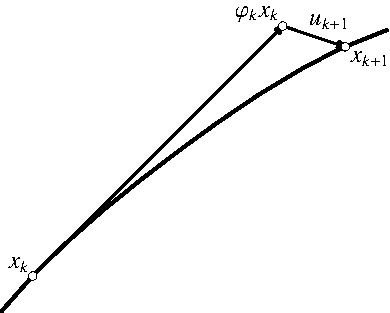
\includegraphics{images/filter-1.pdf}
\caption{Systementwicklung durch die Abbildung $\varphi_k$, der Vektor $u_k$
gibt die Unzul"anglichkeiten des durch $\varphi_k$ implementierten Modells
wieder.
\label{filter-systementwicklung}}
\end{figure}
In der Realtit"at bewegt sich das System kaum genau nach diesen Gleichungen.
Vielmehr wird es von "ausseren St"orungen beeinflusst, die sich einer
exakten Vorhersage entziehen, wir tragen dem Rechnung mit Hilfe eines
zus"atzlichen Zufallsvektors $u_k$ in den Bewegungsgleichungen
\[
x_{k+1}=\varphi_kx_k+ u_k.
\]
Wir verlangen, dass die Komponenten des Vektors $u_k$ alle unabh"angige
Zufallsvariablen sind mit gleicher Varianz, $Q_k=E(u_k\cdot u_k^t)$ ist
ein Mass daf"ur. $u_k$ heisst auch Prozessrauschen oder Systemfehler.

Die Messfehler modellieren wir durch einen
Zufallsvektor $w_k$, der bei jeder Messung dazukommt, also
\[
z_k=H_kx_k+w_k.
\]
Die Komponenten von $w_k$ sollen unabh"angige Zufallsvariablen mit
Erwartungswert $0$ sein, d.~h.~es liegen keine systematischen Messfehler
vor. Dies bedeutet, dass die Matrix
\[
R_k=E(w_kw_k^t)
\]
Diagonalform hat.
Ausserdem sollen die Messfehler unabh"angig vom aktuellen Zustand
sein, in Matrix-Form k"onnen wir dies durch $E(x_kw_k^t)=0$ ausdr"ucken.
Man nennt $w_k$ oft auch das Messrauschen.

Die Messfehler $w_k$ und das Prozessrauschen $u_k$ sollen ebenfalls unabh"angig
sein, also $E(w_ku_k^t)=0$.

Das Filterproblem besteht darin, aus den bekannten Messwerten von $z_0,\dots,z_k$
die bestm"ogliche Sch"atzung $\hat x_k$ zu ermitteln. Dabei sollen
nat"urlich die Bewegungsgleichungen ber"ucksichtigt werden. Da aber
mit der Matrix $R_k$ auch die Gr"ossenordnung der Messfehler bekannt ist,
sollen ``schlechte'' Messwerte geringeres Gewicht erhalten also gute
Messwerte. Je mehr Werte $z_k$ bekannt werden, desto besser sollte die
Sch"atzung werden.

In einer praktischen Realisierung muss aber auch die Berechnung der Sch"atzung
einfach und mit wenig Speicherplatz m"oglich sein. Insbesondere sollte zur
Berechnung der neuen Sch"atzung $\hat x_{k+1}$ nur der letzte bekannte Sch"atzwert
$\hat x_k$ und die Messung $z_{k+1}$ notwendig sein. Ausserdem soll der Sch"atzer
$\hat x_k$ m"oglichst gut sein, d.~h.~erwartungstreu, linear, iterativ und
mit minimaler Varianz.

\begin{definition}Gegeben ist ein lineares System der Zeitentwicklung
\[
x_{k+1}=\varphi_kx_k+u_k
\]
wobei $x_k$ und $u_k$ unkorrellierte Zufallsvariablen sind,
$u_k$ mit Erwartungswert $0$ und bekannter Kovarianzmatrix $Q_k$, d.~h.
\[
E(u_kx_k^t)=0,\qquad E(u_k)=0,\qquad E(u_ku_k^t)=Q_k.
\]
An diesem System werden Beobachtungen
\[
z_k=H_kx_k+w_k
\]
vorgenommen, $w_k$ sind mit $x_k$ und $u_k$ unkorrellierte Zufallsvariablen,
$w_k$ mit Erwartungswert $0$ und bekannter Kovarianzmatrix $R_k$, also
\[
E(w_kx^t)=0,\qquad E(w_k)=0,\qquad E(w_kw_k^t)=R_k.
\]
Das Filterproblem besteht darin, einen Sch"atzer $\hat x_k$ zu
finden, welche sich linear aus $\hat x_{k-1}$ und $z_k$ berechnen l"asst.
Die Fehler $\tilde x_k=\hat x_k-x_k$ k"onnen mit der Fehlerkovarianzmatrix
\[
P_k=E(\tilde x_k\tilde x_k^t)
\]
gemessen werden. Der Sch"atzer soll so gew"ahlt werden, dass die Spur
$\operatorname{tr}P_k$ minimal wird.
\end{definition}

\section{L"osung f"ur das Filterproblem}
Zur Zeit $k$ ist das System im Zustand $x_k$, von dem uns aber nur die
Sch"atzung $\hat x_k$ bekannt ist. Anschliessend wird sich
das System entsprechend der Zeitentwicklungsgleichung entwickeln und
so den Zustand $x_{k+1}$ erreichen. Auch diesen Zustand k"onnen wir nicht
kennen, es gen"ugt, eine Sch"atzung davon zu bestimmen. Dies kann in zwei
Schritten geschehen
\begin{enumerate}
\item Man "uberl"asst das System sich selbst, und versucht eine m"oglichst
gute Sch"atzung f"ur den Zustand $x_{k+1}$ zu finden, die nur auf dem
Wissen zur Zeit $k$ basiert. Wir schreiben daf"ur $\hat x_{k+1|k}$.
\item Mit Hilfe der Messung $z_{k+1}$, die zur Zeit $k+1$ stattfindet, wird
$\hat x_{k+1|k}$ zu einer optimalen Sch"atzung zur Zeit $k+1$ verfeinert.
\end{enumerate}
Tabellarisch k"onnen wir die Schritte wie folgt darstellen:
\[
\xymatrix @-1mm {
k\ar[dd]&x_k\ar[dd]\ar[dd]^{\varphi_k, u_k} &\hat x_k\ar[d]^{\varphi_k}      &P_{k} \ar[d]^{\varphi_k,Q_k}    \\
        &           &\hat x_{k+1|k}\ar[d]^{H_k,K_k}&P_{k+1|k}\ar[d]^{R_k,H_k\Rightarrow K_k} \\
k+1     &x_{k+1}    &\hat x_{k+1}  &P_{k+1}
} \]
Die Pfeile sind mit den Matrizen angeschrieben, die bei den einzelnen Schritten zum
Einsatz kommen werden.

\subsection{Voraussage}
\begin{figure}
\centering
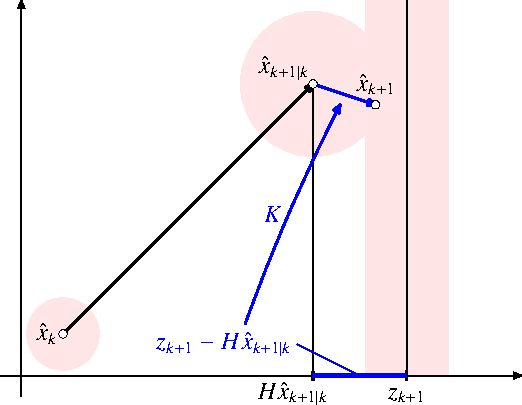
\includegraphics{images/filter-2.pdf}
\caption{Vorhersage und Messung mit ihren jeweiligen Fehlern geben eine
korrigierte Vorhersage h"oherer Genauigkeit
\label{bild-vorhersage-korrektur}}
\end{figure}
"Uberl"asst man das System sich selbst, wird es sich gem"ass der
Entwicklungsgleichung entwickeln. Allerdings ist uns der Systemfehler
$u_k$ nicht bekannt, die einzige Sch"atzung, die uns auf der Basis dieser
Informationen m"oglich ist, ist also
\[
\hat x_{k+1|k}=\varphi_k\hat x_k
\]
In Abbildung~\ref{bild-vorhersage-korrektur} ist die Vorhersage schematisch
dargestellt, zusammen mit ihren Fehlern.

Wir wollen nicht nur $\hat x_k$ zu jeder Zeit bestimmen k"onnen, sondern
auch eine Information "uber die Fehler mitberechnen, also die Fehlerkovarianzmatrix
nachf"uhren. Wir berechnen daher auch $P_{k+1|k}$
\begin{align*}
P_{k+1|k}&=E(\tilde x_{k+1|k}\tilde x_{k+1|k}^t)\\
&=E( (\hat x_{k+1|k}-x_{k+1} ) (\hat x_{k+1|k}-x_{k+1} )^t)\\
&=E(
(\varphi_k\hat x_k-\varphi_kx_k-u_k)
(\dots)^t
)\\
&=E(
(\varphi_k\hat x_k-x_k)-u_k)
(\dots)^t
)\\
&=E(
(\varphi_k(\tilde x_k)-u_k)
(\dots)^t
)\\
&=E(
(\varphi_k(\tilde x_k)-u_k)
(\tilde x_k^t\varphi_k^t-u_k^t)
)\\
&=E(\varphi_k\tilde x_k \tilde x_k^t\varphi_k^t)-E(u_k\tilde x_k\varphi_k^t)-E(\varphi_k\tilde x_ku_k)+E(u_ku_k^t)\\
&=\varphi_k E(\tilde x_k \tilde x_k^t)\varphi_k^t-E(u_k\tilde x_k)\varphi_k^t-\varphi_k E(\tilde x_ku_k)+E(u_ku_k^t)\\
&=\varphi_kP_k\varphi_k^t+Q_k
\end{align*}
Damit haben wir einen Formelsatz, mit dem der erste Teilschritt zur Berechnung
der Sch"atzung zur Zeit $k+1$ m"oglich ist:
\begin{definition}Der Voraussageschritt f"ur das Filterproblem wird durch
\begin{align}
\hat x_{k+1|k}&=\varphi_k\hat x_k \label{estimate-prediction}\\
P_{k+1|k}&=\varphi_kP_k\varphi_k^t + Q_k \label{covariance-prediction}
\end{align}
berechnet.
\end{definition}

\subsection{Korrektur}
Im zweiten Schritt wird jetzt aus der provisorischen Sch"atzung $\hat x_{k+1|k}$
und der Messung $z_{k+1}$ die definitive Sch"atzung zur Zeit $k+1$ berechnet.
Ebenfalls nachgef"uhrt werden muss die Fehlerkovarianzmatrix $P_{k+1}$.
In Abbildung~\ref{bild-vorhersage-korrektur} ist auch die Korrektur auf der Basis
der Messung $z_{k+1}$ dargestellt, so entsteht eine neue Sch"atzung
$\hat x_{k+1}$ h"oherer Pr"azision.

In den folgenden Herleitungen kommt vor allem der Index $k+1$ vor. Um die Formeln
etwas zu vereinfachen, erh"ohen wir jetzt $k$ um eins, d.~h.~wir k"onnen
"uberall $k+1$ durch $k$ und $k$ durch $k-1$ ersetzen.

Da der Sch"atzer linear sein soll, und nur von $\hat x_{k|k-1}$ und $z_{k}$
abh"angen soll, setzen wir ihn mit Hilfe der zwei Matrizen $K_k'$ und $K_k$
wie folgt an:
\[
\hat x_{k}=K_{k}' \hat x_{k|k-1}+K_{k} z_{k}.
\]
Die Matrizen $K_{k}'$ und $K_{k}$ sollen jetzt so bestimmt werden, dass der Sch"atzer
$\hat x_{k}$ gute Eigenschaften hat.

Zun"achst m"ochten wir sicherstellen, dass der Sch"atzer erwartungstreu ist,
oder, was auf das gleiche hinausl"auft, dass der Erwartungswert des Fehlers
$\tilde x_{k}=\hat x_{k}-x_{k}$ verschwindet. Wir berechnen den Fehler
mit Hilfe der Formel f"ur $\hat x_{k}$
\begin{align*}
\tilde x_{k}&=\hat x_{k}-x_{k}\\
&=K_{k}'\hat x_{k|k-1}+K_{k}z_{k}-x_{k}\\
&=K_{k}'\hat x_{k|k-1}+K_{k}H_{k}x_{k} + K_{k}w_{k}-x_{k}\\
&=K_{k}'\hat x_{k|k-1}+K_{k}H_{k}x_{k} -x_{k} + K_{k}w_{k}\\
&=K_{k}'(\tilde x_{k|k-1}+x_{k})+K_{k}H_{k}x_{k}-x_{k}+K_{k}w_{k}\\
&=(K_{k}'+K_{k}H_{k}-I)x_{k}+K_{k}'\tilde x_{k|k-1}+K_kw_k
\end{align*}
Daraus berechnet man den Erwartungswert des Fehlers
\begin{align*}
E(\tilde x_{k})&=(K_{k}'+K_{k}H_{k}-I)E(x_{k})+K_{k}'E(\tilde x_{k|k-1})+K_{k}E(w_{k})\\
&=(K_{k}'+K_{k}H_{k}-I)E(x_{k})
\end{align*}
weil $\tilde x_{k|k-1}$ bereits erwartungstreu ist und $E(w_{k})=0$ nach Voraussetzung.
Dies verschwindet nur dann immer, wenn die Matrix in Klammern $0$ ist,
also
\[
K_{k}'+K_{k}H_{k}-I=0\qquad\Rightarrow\qquad K_{k}'=I-K_{k}H_{k}.
\]
Somit ist $K_{k}'$ durch die Bedingung der Erwartungstreue eindeutig bestimmt.
Mit dieser Wahl von $K_{k}'$ wird der Sch"atzer jetzt
\[
\hat x_{k}=(I-K_{k}H_{k})x_{k|k-1}+K_{k}z_{k}.
\]

Die zweite Bedingung ist, dass die Fehlerkovarianzmatrix m"oglichst klein wird,
daher berechnen wir zun"achst $\tilde x_{k}$:
\begin{align*}
\tilde x_{k}&=\hat x_{k}-x_{k}\\
&=(I-K_{k}H_{k})\hat x_{k|k-1}+K_{k}z_{k}-x_{k}\\
&=(I-K_{k}H_{k})\hat x_{k|k-1}+K_{k}H_{k}x_{k}+K_{k}w_k-x_{k}\\
&=(I-K_{k}H_{k})\tilde x_{k|k-1}+K_{k}w_k
\end{align*}
Somit ist $\tilde x_{k}$ durch $\tilde x_{k|k-1}$ ausgedr"uckt, damit sollten
wir $P_{k}$ aus $P_{k|k-1}$ berechnen k"onnen:
\begin{align*}
P_{k}&=E(\tilde x_{k}\tilde x_{k}^t)\\
&=E(
((I-K_{k}H_{k})\tilde x_{k|k-1}+K_{k}w_k)
(\dots)^t
)\\
&=(I-K_{k}H_{k})P_{k|k-1}(I-K_{k}H_{k})^t\\
&\quad +(I-K_{k}H_{k})E(\tilde x_{k|k-1}w_k^t)K_{k}^t\\
&\quad+K_{k}E(w_k\tilde x_{k|k-1}^t)(I-K_{k}H_{k})\\
&\quad+K_{k}E(w_kw_k^t)K_{k}^t\\
&=(I-K_{k}H_{k})P_{k|k-1}(I-K_{k}H_{k})^t +K_{k}R_kK_{k}^t
\end{align*}
Diese Formeln bilden nun auch den zweiten Schritt, offen ist nur noch die
geeignete Wahl der Matrix $K_{k}$.
\begin{definition}
Der Korrekturschritt im Filterproblem ist gegeben durch
\begin{align}
\hat x_{k}&=(I-K_{k}H_{k})x_{k|k-1}+K_{k}z_{k} \label{estimate-correction}\\
P_{k} &=(I-K_{k}H_{k})P_{k|k-1}(I-K_{k}H_{k})^t +K_{k}R_kK_{k}^t \label{covariance-correction}
\end{align}
\end{definition}

\subsection{Der optimale Filter}
Die Zeitentwicklung des Sch"atzers kann nun bis auf die unbekannte Matrix $K_k$
berechnet werden. Es bleibt, $K_k$ zu bestimmen. $K_k$ soll so gew"ahlt werden,
dass die Spur von $P_{k}$ minimal wird. Dabei k"onnen wir verwenden,
dass $P_{k}$ von der Form $ABA^t$ ist, wobei $B$ eine symmetrische
Matrix ist. F"ur solche Matrizen ist die Ableitung nach den Komponenten
$A$ leicht zu berechnen, das Minimum von $\operatorname{tr}(ABA^t)$
kann daher durch Nullsetzen der Ableitung gefunden werden.

\begin{hilfssatz}Ist $B$ eine symmetrische Matrix und $A$ eine beliebige
Matrix, dann ist die Matrix der Ableitungen von $\operatorname{tr}(ABA^t)$
nach den Komponenten von $A$  ist $2AB$.
\end{hilfssatz}

\begin{proof}[Beweis]
Es ist
\[
\operatorname{tr}(ABA^t)=\sum_{i,j,k}a_{ij}b_{jk}a_{lk}.
\]
Ableiten nach $a_{uv}$ ergibt:
\[
\frac{\partial}{\partial a_{uv}}\operatorname{tr}(ABA^t)
=\sum_{k}b_{vk}a_{uk}+\sum_{j}a_{uj}b_{jv}
\]
Die zwei Terme auf der rechten Seite unterscheiden sich nur durch
die Bezeichnung f"ur die Laufvariable, also
\[
\frac{\partial}{\partial a_{uv}}\operatorname{tr}(ABA^t)
=(2AB)_{uv}.
\]
\end{proof}

Angewendet auf $P_{k}$ bedeutet dies, dass f"ur das optimale $K_k$
\[
-(I-K_kH_{k})P_{k|k-1}H_{k}^t +K_kR_k=0
\]
verlangt werden muss.
Dies kann man nach $K_k$ aufl"osen und findet
\begin{align*}
0&=-P_{k|k-1}H_{k}^t +K_k[H_{k}P_{k|k-1}H_{k}^t +R_{k}]\\
P_{k|k-1}H_{k}^t&=K_k[H_{k}P_{k|k-1}H_{k}^t +R_{k}]\\
K_k&= P_{k|k-1}H_{k}^t [H_{k}P_{k|k-1}H_{k}^t +R_{k}]^{-1}
\end{align*}
Damit ist das Filterproblem eigentlich vollst"andig gel"ost. Wir bem"uhen uns
aber noch, mit der L"osung f"ur $K_k$ die Berechnung der Fehlerkovarianz etwas zu
vereinfachen.
Es gilt
\begin{align*}
P_{k}&=(I-K_{k}H_{k})P_{k|k-1}(I-K_{k}H_{k})^t+K_{k}R_kK_{k}^t\\
&=P_{k|k-1} + K_{k}(H_{k}P(-)H_{k}^t+R_k)K_{k}^t -K_{k}H_{k}P_{k|k-1}-P_{k|k-1}H_{k}^tK_{k}^t\\
&=P_{k|k-1} - P_{k|k-1}H_{k}^t(H_{k}P_{k|k-1}H_{k}^t+R_k)^{-1}H_{k}P_{k|k-1}\\
&=(I-P_{k|k-1}H_{k}^t(H_{k}P_{k|k-1}H_{k}^t + R)^{-1}H_{k})P_{k|k-1}\\
&=(I-K_{k}H_{k})P_{k|k-1}\\
\end{align*}
Damit k"onnen wir das Resultat zusammenstellen:
\begin{satz}
Der beste lineare Sch"atzer f"ur das Filterproblem wird durch die Kalman-Matrix
$K_k$ gegeben, welche mittels
\begin{equation}
K_k=P_{k|k-1}H_k^t(H_kP_{k|k-1}H_k^t+R_k)^{-1}
\label{kalman-gains}
\end{equation}
berechnet wird. Das Fehlerkovarianz-Update wird mit der Kalman-Matrix
vereinfacht zu
\[
P_k=(I-K_kH_k)P_{k|k-1}.
\]
\end{satz}

\subsection{Datenfluss}
\begin{figure}
\[
\xymatrix @-1mm {
&u_k\ar[r]& *+[o][F]{+}\ar[ddd]_{x_k}&                               \\
&&                   & *+[F]{\varphi_{k-1}}\ar `u^l[ul] [ul]          \\
*\txt{unbeobachtetes System}&&                   & *+[F]\txt{DELAY} \ar[u]       \\
&& *{\bullet}\ar[dd]\ar `r^u[ru] [ru]         &                        \\
\ar@{.}[rrr]&&&\\
*\txt{Messung}&& *+[F]{H_k}\ar[d] & \\
&w_k\ar[r]& *+[o][F]{+}\ar[dd]_<<<<{z_k} &                      \\
\ar@{.}[rrr]&&&\\
&& *+[o][F]{-}\ar[d]_{z_k-H_k \hat x_{k|k-1}} &                               \\
&& *+[F]{K_k}\ar[d]  & *+[F]{H_k}\ar `u^l[ul] [ul]   \\
*\txt{Kalman-Filter}&& *+[o][F]{+}\ar[ddd]_{\hat x_k}  & *{\bullet}\ar[u]\ar[l]\\
&&                   & *+[F]{\varphi_{k-1}}\ar[u]^{\hat x_{k|k-1}}            \\
&&                   & *+[F]\txt{DELAY} \ar[u]       \\
&& *{\bullet}\ar `r^u[ru] [ru] \ar[d]&                     \\
&& \hat x_k          &                               \\
}\]
\caption{Datenfluss im Kalman-Filter\label{datenfluss}}
\end{figure}
\begin{figure}
\[
\xymatrix @-1mm {
*+[F]{H_{k-1}}\ar [rd] & & \\
&*+[F]\txt{Berechne $P_{k-1}$ nach (\ref{covariance-correction})}\ar[ddd]&\\
*+[F]{R_{k-1}}\ar[ur] & & \\
*+[F]{\varphi_{k-1}}\ar[dr] & & \\
&*+[F]\txt{Berechne $P_{k|k-1}$ nach (\ref{covariance-prediction})} \ar[dd] & &\\
*+[F]{Q_{k-1}} \ar[ur] & & \\
&*[F]\txt{\strut Berechne $K_k$ nach (\ref{kalman-gains})} \ar[d] && \\
&*{\bullet} \ar `r^u[r] `u^l[ruuuuuuu]_{\text{erh"ohe }k} `l^d[uuuuuuu] [uuuuuu] \ar[d]&&\\
&&&\\
}\]
\caption{Berechnung der Kalman-Matrix\label{k-berechnung}}
\end{figure}
Abbildung \ref{datenfluss} zeigt den Datenfluss f"ur den Kalman Filter.
Im oberen Teil des Diagrams ist das `unbeobachtete' System mit seiner
Zeitentwicklung und den Systemfehlern $u_k$ dargestellt. Unterhalb der
punktierten Linie folgt die Messung, die Matrix $H_k$ reduziert den Zustand
auf diejenigen Gr"ossen, die durch die Messung zug"anglich werden, und es
werden die Messfehler $w_k$ hinzugef"ugt. Beide Teile sind nur f"ur die
mathematische Beschreibung des Kalman-Filters notwendig, sie werden
sozusagen von der Natur und den Sensoren realisiert.

Die untere H"alfte zeigt den eigentlichen Kalman-Filter.
Aus einem fr"uhren Zustand $\hat x_{k-1}$ wird mit Hilfe der Matrix
$\varphi_k$ eine provisorische Sch"atzung $\hat x_{k|k-1}$ erstellt.
Mit der Matrix $H_k$ wird darauf eine Messung simuliert. Diese wird
mit der tats"achlichen Messung verglichen und die Differenz, verst"arkt durch
die Kalman-Matrix $K_k$ zur provisorischen Sch"atzung hinzugef"ugt, was
die definitive neue Sch"atzung $\hat x_k$ f"ur $x_k$ ergibt.

In Abbildung \ref{k-berechnung} ist der Datenfluss f"ur die Berechnung
der Fehlerkovarianzmatrix und der Kalman-Matrix dargestellt.

\subsection{Spezialf"alle}
Sind die Matrizen konstant, die das System und den Messprozess beschreiben, 
dann werden im Prozess nach Abbildung \ref{k-berechnung} sowohl $P_k$ also auch
$K_k$ oft gegen konstante Matrizen konvergieren. In diesem Fall kann man
die Matrix $K=\lim_{n\to\infty}K_n$ vorg"angig berechnen, und braucht
in der Implementation des Filters die Berechnung der Fehlerkovarianzmatrix
gar nicht mehr mitzuberechnen. 

Wir betrachten den Spezialfall eines konstanten System mit genau einer
Zustandsvariable,
die auch gemessen wird. Man erwartet keine "Anderung der Zustandsvariable,
die Matrix $\varphi$ ist also die Einheitsmatrix. Der Voraussageschritt wird
dann zu 
\begin{align*}
\hat x_{k|k-1}&=\hat x_{k-1}\\
P_{k|k-1}&=P_{k-1}+Q,
\end{align*}
die Kalman-Matrix 
\[
K_{k}=\frac{P_{k|k-1}}{P_{k|k-1}+R}=\frac{P_{k-1}+Q}{P_{k-1}+Q+R},
\]
und das Update der Fehlerkovarianz damit zu
\begin{align*}
P_k&=(1-K_k)P_{k|k-1}\\
&=\frac{R(P_{k-1}+Q)}{P_{k-1}+Q+R}
\end{align*}
Diese Gleichung hat tats"achlich einen Fixpunkt, den man durch
Einsetzen von $P=P_k=P_{k-1}$ findet:
\[
P=\frac{R(P+Q)}{P+Q+R}
\quad\Rightarrow\quad
P^2+QP-QR=0
\quad\Rightarrow\quad
P=\frac{Q}2+\sqrt{\frac{Q^2}4+RQ}
\]
Damit kann man nun auch einen geschlossenen Ausdruck f"ur $K$
finden:
\[
K=\frac{1}{1+R\biggl(\displaystyle\frac{Q}2+\sqrt{\frac{Q^2}4+RQ}\biggr)^{-1}}
=\frac1{1+R/P}
\]
Wir beobachten darin folgende Grenzf"alle:
\begin{enumerate}
\item Ist $R=0$, also keine Messfehler, dann ist $K=1$. Da die Vorhersage
$\hat x_{k|k-1}=\hat x_k$ ist, bedeutet dies, dass Abweichungen des Messwertes
von der Vorhersage vollst"andig in den neuen Messwert "ubernommen werden,
der Kalmanfilter reproduziert also die Messwerte exakt.
\item Im Grenzfall $Q=0$ erhalten wir $P=0$ und damit auch $K=0$. Dies
bedeutet, dass der Filter "uberhaupt nicht mehr auf die Messungen reagiert,
der einmal ermittelte Sch"atzwert ist bereits die beste m"ogliche Sch"atzung.
\item F"ur einen Zwischenwert ergibt sich ein Wert von $K$ zwischen $0$ und $1$.
Nehmen wir als Beispiel an, dass die Messwerte bei $k_0$ einen Sprung machen,
danach aber konstant sind, dann wird der Sch"atzwert gegen den neuen Messwert
konvergieren. Die Abweichung zwischen Messwert und vorhergesagtem Wert wird
in jeder Iteration mit $K$ multipliziert. Bei einem kleinen Wert von $K$
kann der Filter einer "Anderung rascher folgen, daf"ur wird auch $P$ entsprechend
gross, die Sch"atzung ist also nicht besonders zuverl"assig.
Umgekehrt wird der Filter mit $K$ nahe bei $1$ tr"age, daf"ur kann dann auch
$P$ kleiner sein, die Sch"atzungen des Filters sind pr"aziser.
\end{enumerate}
Auch im allgemeinen Fall eines konstanten Systems kann man erwarten,
dass bei einem Sprung der Inputdaten der Filter eine Abweichung vom
wahren Wert zeigt, welche exponentiell zerf"allt.

\section{Beispiel: Positionsmessung und Geschwindigkeit}
\begin{figure}
\centering
\includegraphics{tacho/graph-1.pdf}
\caption{Kalman-Filter zur Ortsmessung (oben) und Geschwindigkeitsbestimmung
(unten).
Die reale Position ({\color{blue}blau}) wird mit relativ grossem
Fehler gemessen ({\color{green}gr"un}), doch der Filter ({\color{red}rot})
kann die Position rekonstruieren, und sogar einigermassen brauchbare
Werte f"ur die Geschwindigkeit ableiten.
Ebenfalls dargestellt sind die Diagonalelemente der Fehlerkovarianz,
der Positionsfehler ist allerdings 3-fach "uberh"oht.
\label{tacho-graph}}
\end{figure}

\section{Beispiel: H"ohenmesser mit Scheitelpunktermittlung}
Modellraketen verwenden oft einen elektronischen H"ohenmesser, der die H"ohe
barometrisch mit Hilfe eines Drucksensors bestimmt. Die fliegende Modellrakete
kann in erster N"aherung als Massepunkt behandelt werden, der nur unter dem
Einfluss der konstanten Schwerkraft fliegt. Der Systemzustand besteht
dann aus H"ohe $h$, Vertikalgeschwindigkeit $v$ und Beschleunigung $a$.
Die Kinematik beschreibt die zeitliche "Anderung mit Hilfe des
Differentialgleichungssystems
\[
\frac{d}{dt}
\begin{pmatrix}
h\\v\\a
\end{pmatrix}
=
\begin{pmatrix}
0&1&0\\
0&0&1\\
0&0&0
\end{pmatrix}
\begin{pmatrix}
h\\v\\a
\end{pmatrix}
\]
Die Entwicklungsgleichung f"ur einen Zeitschritt der L"ange $\Delta t$ ist
\[
\varphi=\begin{pmatrix}
1&\Delta t&\frac{\Delta t^2}2\\
0&1&\Delta t\\
0&0&1\\
\end{pmatrix}
\]
Wir nehmen an, dass die Systemfehler, also die Matrix $Q$ ebenfalls diagonal sind,
und alle Komponenten den gleichen Fehler $\sigma^2$ haben, also
\[
Q=\begin{pmatrix}
\sigma^2&0&0\\
0&\sigma^2&0\\
0&0&\sigma^2\\
\end{pmatrix}
\]

Mit dem Drucksensor kann nur die H"ohe bestimmt werden, also
\[
H=\begin{pmatrix}1&0&0\end{pmatrix}
\]
und entsprechend ist die Matrix $R_k$ ebenfalls nur eine Zahl, welche
den Messfehler $\varrho^2$ der Messung wiedergibt.

Zur Berechnung der Kalmanmatrix muss die Matrix $HP_{k+1|k}H^t+R$ invertiert werden.
Aber $HP_{k+1|k}H^t$ ist einfach nur die Zahl in der linken oberen Ecke, also
der mittlere quadratische Sch"atzfehler der H"ohe. Das Produkt $P_{k+1|k}H^t$
ist die erste Spalte der Kovarianzmatrix. Die Kalmanmatrix ist also die erste
Spalte der Kovarianzmatrix dividiert durch $(P_{k+1|k})_{11}+\rho^2$.

\section{Bedingte Erwartung}
Man h"atte das Filterproblem auch allgemeiner formulieren k"onnen: Es soll
der Erwartungswert des Zustandes bestimmt werden unter Ber"ucksichtigung
der Messungen bis zum Zeitpunkt $k$.
F"ur Wahrscheinlichkeiten wurde dieses
Konzept der Wahrscheinlichkeit unter zus"atzlichen Bedingungen bereits
behandelt. F"ur Erwartungswerte und Verteilungen haben wir bisher keinen
Begriff daf"ur entwickelt.
Man kann zeigen, dass dieser allgemeinere Ansatz zu den gleichen Filtern
f"uhrt. Er bringt uns f"ur unsere Anwendungsf"alle nichts neues, zeigt
aber Erweiterungsm"oglichkeiten der Theorie auf.

Wir haben also zun"achst folgendes Grundproblem zu l"osen: Gegeben sind
zwei Zufallsvariablen $X$ und $Y$. $X$ beschreibt zum Beispiel den vollst"andigen
Systemzustand, $Y$ ist das Resultat einer Messung des Zustandes, sie zeigt
nur ein partielles Bild des Systemzustandes. Welchen Wert von $X$ k"onnen
wir erwarten unter der Voraussetzung, dass ein bestimmter Wert f"ur $Y$
gemessen wurde. Im Kapitel~\ref{chapter-ereignisse-und-wahrscheinlichkeit}
haben wir die bedingte Wahrscheinlichkeit kennengelernt, mit welcher wir
die Wahrscheinlichkeit eines Ereignisses berechnen konnten unter der
Voraussetzung, dass ein anderes Ereignis bereits eingetreten ist. Wenn es
"oglich ist, solche Wahrscheinlichkeiten zu berechnen, dann sollte es auch
m"oglich sein, einen Erwartungswert $E(X|Y=y)$ zu bestimmen. F"ur eine
Beobachtung $y$ der Zufallsvariable $Y$ soll der Ausdruck $E(X|Y=y)$ den
zu erwartenden Wert $X$ liefern. Offensichtlich ist dies eine Funktion,
die bedingte Erwartung, man schreibt sie auch $E(X|Y)\colon y\mapsto E(X|Y=y)$.

Etwas konkreter stellen wir uns als Beispiel einen Scooter mit zuf"alligen
Koordinaten $(X,Y)$ vor, welcher innerhalb eines Dreiecks mit den Ecken
$0$, $(0,1)$ und $(1,0)$ gleichverteilt ist. Allerdings kann man den Scooter
nicht direkt beobachten. Stattdessen ist entlang der $y$-Achse eine
Leinwand aufgespannt, eine Lichtquelle projiziert den Scooter auf diese Leinwand,
es ist also immer nur $Y$ bekannt. Wird f"ur $Y$ der Wert $y$ beobachtet,
schr"ankt dies den Bereich f"ur die m"oglichen $X$-Werte auf das
Intervall $[0,1-y]$ ein.
Innerhalb des m"oglichen Intervalls wird $X$ aber gleichverteilt sein.
Der Erwartungswert von $X$ unter diesen Voraussetzungen ist der Erwartungswert
einer Gleichverteilung auf dem Intervall $[0,1-y]$, also
\[
E(X|Y=y)=\frac{1-y}2
\]
Die bedingte Erwartung $E(X|Y)$ ist also die Funktion
\[
E(X|Y)\colon y\mapsto E(X|Y=y)=\frac{1-y}2.
\]

Allgemeiner nehmen wir an, dass wir die Verteilung von $X$ und $Y$ durch
eine gemeinsame Wahrscheinlichkeitsdichte $\varphi_{X,Y}(x,y)$ beschreiben
k"onnen. Mit ihr ist es m"oglich, die Wahrscheinlichkeit daf"ur zu berechnen,
dass $(X,Y)$ in einem bestimmten Rechteck der Ebene zu finden ist:
\[
P(a\le X\le b\wedge c\le Y\le d)=\int_a^b\int_c^d\varphi_{X,Y}(x,y)\,dy\,dx
\]
Daraus l"asst sich auch die Wahrscheinlichkeitsdichte von $Y$ alleine
berechnen:
\begin{equation}
\varphi_Y(y)=\int_{-\infty}^\infty \varphi_{X,Y}(x,y)\,dx
\label{dichtefunktion-von-Y-alleine}
\end{equation}
Wir m"ochten jetzt die bedingte Erwartung $E(X|Y=y)$ berechnen. Dazu brauchen
wir zun"achst die Wahrscheinlichkeiten f"ur die verschiedenen Werte von $X$
unter der Voraussetzung, dass $Y=y$ ist.
Die Theorie der bedingten Wahrscheinlichkeit sagt dazu
\[
P(A|Y=y)=\frac{P(A\cap \{Y=y\})}{P(\{Y=y\})},
\]
was ungl"ucklicherweise f"ur eine stetige Wahrscheinlichkeitsverteilung
wegen $P(Y=y)=0$ sinnlos ist. Wir k"onnten in diesem Falle aber die
Wahrscheinlichkeit daf"ur bestimmen, dass $(X|Y)$ in einem sehr schmalen
Streifen $\mathbb{R}\times [y-\varepsilon, y+\varepsilon]$ zu finden ist.
Beim Grenz"ubergang $\varepsilon\to0$ erwarten wir, wieder einen sinnvollen
Wert f"ur die bedingte Wahrscheinlichkeit:
\begin{align*}
P(a\le X\le b|Y=y)
&=
\lim_{\varepsilon\to 0} P(a\le X\le b|y-\varepsilon<Y<y+\varepsilon)\\
&=
\lim_{\varepsilon\to 0}
\frac{\int_a^b \int_{y-\varepsilon}^{y+\varepsilon} \varphi_{X,Y}(x,\eta)\,d\eta\,dx}{\int_{y-\varepsilon}^{y+\varepsilon}\varphi_Y(\eta)\,d\eta}\\
&=
\lim_{\varepsilon\to 0}
\int_a^b \frac{\varphi_{X,Y}(x,y)}{\varphi_Y(y)}\,dx
\end{align*}
Dabei sind wir "uber die Grenzwertbildung etwas salopp hinweg gegangen,
mindestens f"ur stetige Funktionen $\varphi_{X,Y}$ und $\varphi_Y$ ist
der Grenz"ubergang zul"assig, er kann aber auch unter weit weniger
restriktiven Bedingungen durchgef"uhrt werden. Damit l"asst sich aus
den Dichtefunktionen eine Wahrscheinlichkeitsverteilung f"ur die
``bedingte Zufallsvariable'' $X|Y=y$ konstruieren, wir fassen diese
Resultate in einem Satz zusammen.

\begin{satz}
\label{bedingte-wahrscheinlichkeitsdichte}
Ist $\varphi_{X,Y}(x,y)$ die gemeinsame Verteilungsfunktion von $X$ und $Y$,
und $Y$ wie in (\ref{dichtefunktion-von-Y-alleine}), dann ist die
Wahrscheinlichkeitsdichte von $X|Y=y$
\[
\varphi_{X|Y=y}(x)=\frac{\varphi_{X,Y}(x,y)}{\varphi_Y(y)},
\]
die bedingte Erwartung ist
\[
E(X|Y=y)=\int_{-\infty}^\infty x\,\frac{\varphi_{X,Y}(x,y)}{\varphi_Y(y)}\,dx.
\]
\end{satz}

In der Praxis hat man meist mit der Situation zu tun, dass im Laufe der Zeit
immer mehr Messungen $y_1,\dots,y_n$ anfallen, es ist ist dann
$E(X|Y_1=y_1\wedge\dots\wedge Y_n=y_n)$ zu bestimmen. Man kann dies auch so
formulieren, dass $y$ ein $n$-dimensionaler Vektor $y\in\mathbb{R}^n$ ist,
die Formeln in Satz \ref{bedingte-wahrscheinlichkeitsdichte} bleiben
dabei unver"andert.

